\documentclass{beamer}

\usepackage[english]{babel}
\usepackage[utf8x]{inputenc}
\usepackage[T1]{fontenc}
\usepackage{lmodern}

%------ tikZ ------%
\usepackage{tikz}
\usetikzlibrary{positioning, arrows}
\usetikzlibrary{backgrounds}

%------------------%
\usepackage{ifthen}
\begin{document}
\begin{frame}
    \frametitle{Convolution operation on an input image with 3 channels (RGB)}
    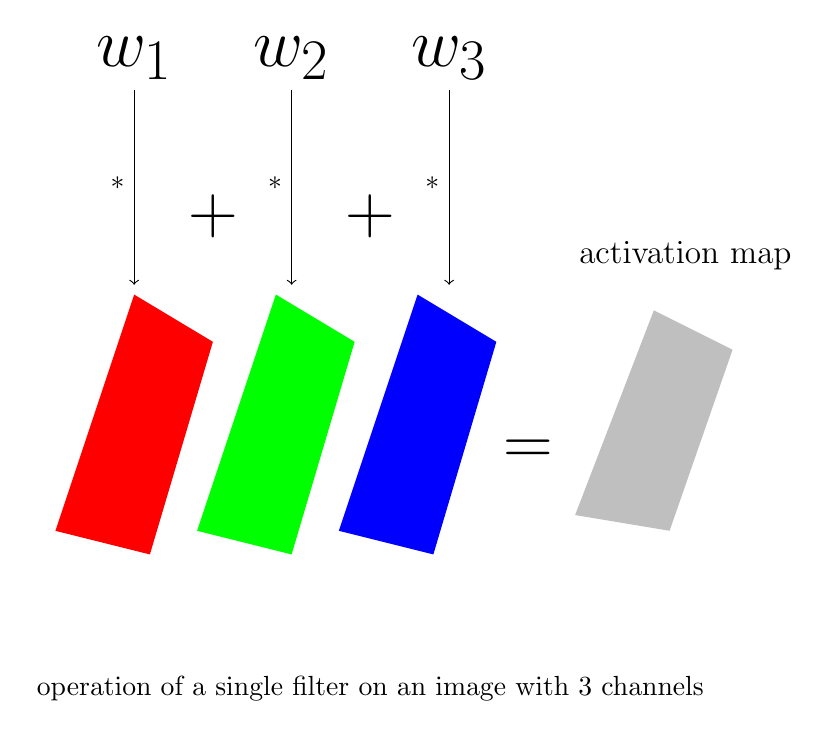
\begin{tikzpicture}
        \node (w1) at (1,6) {\Huge $w_1$};
        \node (w2) at (3,6) {\Huge $w_2$};
        \node (w3) at (5,6) {\Huge $w_3$};
        \node (anc1) at (1,3) {};
        \node (anc2) at (3,3) {};
        \node (anc3) at (5,3) {};
        \node (add1) at (2,4) {\Huge +};
        \node (add2) at (4,4) {\Huge +};
    
        \path[->] (w1) edge node[left]{*} (anc1);
        \path[->] (w2) edge node[left]{*} (anc2);
        \path[->] (w3) edge node[left]{*} (anc3);
    
        \coordinate (a) at (0,0);
         \coordinate (b) at (1,3);
         \coordinate (c) at (2,2.4);
         \coordinate (d) at (1.2,-0.3);
        \filldraw[draw=none,fill=red] (a) -- (b) -- (c) -- (d) -- (a);
    
    
        \coordinate (a1) at (1.8,0);
        \coordinate (b1) at (2.8,3);
        \coordinate (c1) at (3.8,2.4);
        \coordinate (d1) at (3,-0.3);
       \filldraw[draw=none,fill=green] (a1) -- (b1) -- (c1) -- (d1) -- (a1);
        %\filldraw[fill=red] (a) circle (2);
    
        \coordinate (a2) at (3.6,0);
        \coordinate (b2) at (4.6,3);
        \coordinate (c2) at (5.6,2.4);
        \coordinate (d2) at (4.8,-0.3);
       \filldraw[draw=none,fill=blue] (a2) -- (b2) -- (c2) -- (d2) -- (a2);
        %\filldraw[fill=red] (a) circle (2);
    
    \node (eq) at (6,1) {\Huge =};
        \coordinate (a3) at (6.6,0.2);
        \coordinate (b3) at (7.6,2.8);
        \coordinate (c3) at (8.6,2.3);
        \coordinate (d3) at (7.8,0);
       \filldraw[draw=none,fill=lightgray] (a3) -- (b3) -- (c3) -- (d3) -- (a3);
       \node (label) at (4,-2) {operation of a single filter on an image with 3 channels};
       \node (amap) at (8,3.5) {\large activation map};
    \end{tikzpicture}
    

\end{frame}
\begin{frame}[c]
\frametitle{Conv operation on one channel}
\begin{center}
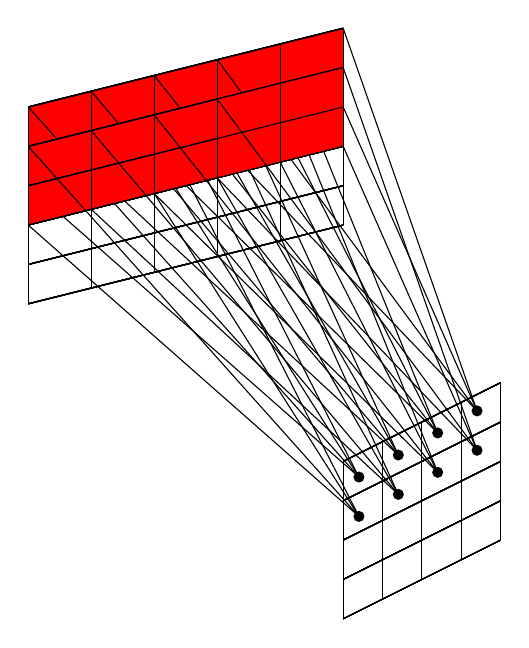
\begin{tikzpicture}
\pgfmathtruncatemacro\N{10}
\foreach \j in {1,...,8}{
    \onslide<\j>{
        \pgfmathsetmacro{\dx}{
            \j<5 ? (0.8*(\j-1)): (0.8*(\j-5))
            }
        \pgfmathsetmacro{\dy}{
            \j<5 ? (0.2*(\j-1)): (0.2*(\j-5)-0.5)
            }
        \pgfmathsetmacro{\tmp}{
            \j<5 ? (8) : (9)
        }
        %\begin{scope}[on background layer]
            \coordinate (a) at (0+\dx,3+\dy);
            \coordinate (d) at (0+\dx ,2+ \dy);
            \coordinate (b) at (1.6+\dx ,3.4+\dy);
            \coordinate (c) at (1.6+\dx,2.4+ \dy);
            \filldraw[fill=red,draw=none] (a) -- (b) -- (c) -- (d) --(a);
        %\end{scope}
        %\node[rectangle,draw] (r) at (\j,\j) {};

          \foreach \k in {1,...,6}
          {
          \pgfmathsetmacro{\idx}{0.2*(\k-1)}
          \pgfmathsetmacro{\sep}{0.8*(\k-1)}


          %horizontal lines
          \path[draw] (0,0.5*\k) -- (4,0.5*\k+1);
          %vertical lines
          \path[draw] (\sep,3+\idx) -- (\sep,0.5+\idx);

          }
          \foreach \k in {1,...,5}
          {
          \pgfmathsetmacro{\idx}{0.25*(\k-1)}
          \pgfmathsetmacro{\sep}{0.5*(\k-1)}


          %horizontal lines
          \path[draw] (4,0.5*\k-4) -- (6,0.5*\k+1-4);
          %vertical lines
          \path[draw] (4+\sep,-1.5+\idx) -- (4+\sep,-3.5+\idx);

          }
          \pgfmathsetmacro{\ccx}{
            \j<5 ? (4.2+0.5*(\j-1)): (4.2+0.5*(\j-5))
            }
            \pgfmathsetmacro{\ccy}{
                \j<5 ? (-1.7+0.28*(\j-1)): (-2.2+0.28*(\j-5))
                }
          \fill (\ccx,\ccy) circle (2pt);
          \path[draw] (a) -- (\ccx,\ccy);
          \path[draw] (b) -- (\ccx,\ccy);
          \path[draw] (c) -- (\ccx,\ccy);
          \path[draw] (d) -- (\ccx,\ccy);
    }
}

\end{tikzpicture}
\end{center}

\end{frame}


%% bottom part
\begin{frame}[c]
    \frametitle{Conv operation on one channel}
    \begin{center}
    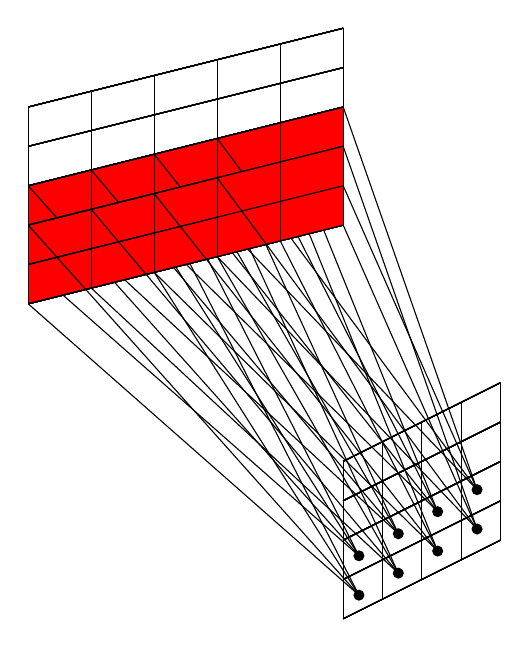
\begin{tikzpicture}
    \pgfmathtruncatemacro\N{10}
    \foreach \j in {1,...,8}{
        \onslide<\j>{
            \pgfmathsetmacro{\dx}{
                \j<5 ? (0.8*(\j-1)): (0.8*(\j-5))
                }
            \pgfmathsetmacro{\dy}{
                \j<5 ? (0.2*(\j-1)): (0.2*(\j-5)-0.5)
                }
            \pgfmathsetmacro{\tmp}{
                \j<5 ? (8) : (9)
            }
                \coordinate (a) at (0+\dx,2+\dy);
                \coordinate (d) at (0+\dx ,1+ \dy);
                \coordinate (b) at (1.6+\dx ,2.4+\dy);
                \coordinate (c) at (1.6+\dx,1.4+ \dy);
                \filldraw[fill=red,draw=none] (a) -- (b) -- (c) -- (d) --(a);
          
              \foreach \k in {1,...,6}
              {
              \pgfmathsetmacro{\idx}{0.2*(\k-1)}
              \pgfmathsetmacro{\sep}{0.8*(\k-1)}
    
    
              %horizontal lines
              \path[draw] (0,0.5*\k) -- (4,0.5*\k+1);
              %vertical lines
              \path[draw] (\sep,3+\idx) -- (\sep,0.5+\idx);
    
              }
              \foreach \k in {1,...,5}
              {
              \pgfmathsetmacro{\idx}{0.25*(\k-1)}
              \pgfmathsetmacro{\sep}{0.5*(\k-1)}
    
    
              %horizontal lines
              \path[draw] (4,0.5*\k-4) -- (6,0.5*\k+1-4);
              %vertical lines
              \path[draw] (4+\sep,-1.5+\idx) -- (4+\sep,-3.5+\idx);
    
              }
              \pgfmathsetmacro{\ccx}{
                \j<5 ? (4.2+0.5*(\j-1)): (4.2+0.5*(\j-5))
                }
                \pgfmathsetmacro{\ccy}{
                    \j<5 ? (-2.7+0.28*(\j-1)): (-3.2+0.28*(\j-5))
                    }
              \fill (\ccx,\ccy) circle (2pt);
              \path[draw] (a) -- (\ccx,\ccy);
              \path[draw] (b) -- (\ccx,\ccy);
              \path[draw] (c) -- (\ccx,\ccy);
              \path[draw] (d) -- (\ccx,\ccy);
        }
    }
    
    \end{tikzpicture}
    \end{center}
    
    \end{frame}
    

    \begin{frame}
        \frametitle{Example: Conv. operation on one channel}
      \vspace{-1cm}
      
      
          \begin{tabular}[h]{|c|c|c|c|}
            \multicolumn{4}{c}{Input}\\
            \hline
             {\only<1>{\color{red}} 1}& {\only<1-2>{\color{red}} 2} &  {\only<2-3>{\color{red}} 4}&  {\only<3>{\color{red}} 3}\\
            \hline
               {\only<1,4>{\color{red}} 5}&{\only<1-2,4-5>{\color{red}} 6}& {\only<2-3,5-6>{\color{red}} 8}&{\only<3,6>{\color{red}} 7}\\
           \hline
               {\only<4,7>{\color{red}} 9}&{\only<4-5,7-8>{\color{red}} 10}  &{\only<5-6,8-9>{\color{red}} 12}&{\only<6,9>{\color{red}} 11}\\
           \hline
              {\only<7>{\color{red}} 13}&{\only<7-8>{\color{red}} 14} &{\only<8-9>{\color{red}} 16} &{\only<9>{\color{red}} 2}\\
           \hline
          \end{tabular}
      \hspace{0.5cm}$\odot$\hspace{0.5cm}
          \begin{tabular}[h]{|c|c|}
            \multicolumn{2}{c}{Kernel}\\
            \hline
             1 &-2 \\
            \hline
             -3 & 4\\
             \hline
          \end{tabular}
      
      
      \vspace{1cm}
      \hspace{4.5cm}
      =
      %\onslide<2>{
      \begin{tabular}[h]{|c|c|c|}
        \hline
         \only<1-> 6& \only<2-> 8 &\only<3-> {2}\\
        \hline
        \only<4-> 6  &\only<5-> 8 &\only<6->2\\
        \hline
        \only<7-> 6 &\only<8-> 8 &\only<9-> {-50}\\
        \hline
      \end{tabular}
      \tikz{
        \node[overlay] at (-1,1.2) {activation map};

      }
      
      \end{frame}
\begin{frame}
    \frametitle{Stride, receptive field, and Padding}
\begin{itemize}
    \item In the previous example we used a \textbf{stride} equal to 1
    \item The kernel \textbf{receptive field} was equal to 2x2
    \item The size of the output (activation map) was 3x3
    \item Are those numbers the same in all applications? No
\end{itemize}
    

\end{frame}  
\begin{frame}
    \frametitle{Stride, receptive field, and Padding}
\begin{itemize}
    \item In general one can use a stride of any size $S$. Stride of size 1 is the most common.
    \item When the stride is larger than 1 we might need \textbf{padding}
    \item Let $F\times F$ be the kernel \textbf{receptive field} 
    \item Let $H_i\times W_i\times C_i$ be the size of the input
    \item The size of the resulting activation map is $H_o\times W_o$ where 
    \begin{align*}
        H_o&=\frac{H_i-F+2P}{S}+1\\
        W_o&=\frac{W_i-F+2P}{S}+1
    \end{align*}
\end{itemize}
    

\end{frame}      
\begin{frame}
    \frametitle{Convolution operation mathematically}

    Let $s,i,j,f$ be the number of samples,output height index,output width index, and the filter index respectively. The convolution operation is defined as
\begin{align*}
O_{s,f,i,j}=\sum_c\sum_{m,n}X_{s,c,i+m,j+n}*K_{f,c,m,n}
\end{align*}

\end{frame}
\end{document}